\documentclass[11pt]{article}
\usepackage[margin=1in]{geometry}
\usepackage{graphicx}
\usepackage{booktabs}
\usepackage{array}
\usepackage{float}
\usepackage{amsmath}
\usepackage{hyperref}

\title{Numerical Reliability Audit for the Discovery Active-Learning Phase Diagram}
\author{}
\date{May 23, 2026}

\begin{document}
\maketitle

\section*{Purpose}

This note consolidates the numerical checks performed after the discovery-mode
active-learning run
\[
\texttt{active\_boundary\_discovery\_512seed\_256x50}.
\]
The active-learning loop found the main thermodynamic phase structure from
random exact seeds, but several high-\(J_A\), low-temperature regions required
additional numerical scrutiny.  The checks summarized here are audit-only:
they do not modify the active-learning data set, the acquisition function, the
neural-network surrogate, the StopController, or the production BdG oracle.

The central questions are:

\begin{enumerate}
  \item Is the normal/SC and uniform-SC/FFLO phase labeling reliable near the
        high-\(J_A\), low-\(T\) boundary region?
  \item Are the apparent high-\(J_A\), positive-\(\eta\) points robust diode
        responses or numerical response-extraction artifacts?
  \item What numerical issues remain unresolved before treating the high-\(J_A\)
        response and branch structure as final physics?
\end{enumerate}

\section*{Free-energy phase criterion}

At each point \((k_B T/t,J_A/t)\), the exact solver scans superconducting
ansatz states over \((\Delta,q)\) and compares the best positive-\(\Delta\)
candidate to the normal state:
\[
\Delta F_{\min}
= \min_{\Delta>0,q}\left[F(\Delta,q)-F_N\right].
\]
The phase rule is:
\[
\Delta F_{\min} < -\epsilon_F,\quad \Delta_{\rm opt}>\Delta_\epsilon
\quad \Rightarrow\quad \text{superconducting},
\]
\[
\Delta F_{\min} > +\epsilon_F \ \text{or}\ \Delta_{\rm opt}=0
\quad \Rightarrow\quad \text{normal}.
\]
If \(|\Delta F_{\min}|\) is within tolerance, or if the best positive
\(\Delta\) state is extremely close to the normal state, the point is treated
as boundary-band or ambiguous rather than silently assigned a hard phase.
Within the superconducting sector, the winning \(q_{\rm opt}\) distinguishes
uniform SC and FFLO:
\[
|q_{\rm opt}|\le q_0 \Rightarrow \text{uniform SC}, \qquad
|q_{\rm opt}|>q_0 \Rightarrow \text{FFLO}.
\]

This criterion is physically correct within the scanned numerical window.
The remaining risk is coverage: if the chosen \(q\)-window misses a lower-energy
superconducting branch, the code can find only the window-local minimum.  A
\(q_{\rm opt}\)-edge check reduces this risk, but it cannot prove that another
lower FFLO branch does not exist outside the scanned window.

\section*{Discovery run and revised exact phase diagram}

The discovery run used random initial exact points, full-domain candidate
selection, and stochastic acquisition sampling.  It stopped after discovering
stable main thermodynamic boundaries.  The final exact sample count was
approximately \(5107\) in the reported run.  The selected points became strongly
boundary-focused relative to a random baseline, and the final report recorded
converged main phase boundaries.

\begin{figure}[H]
  \centering
  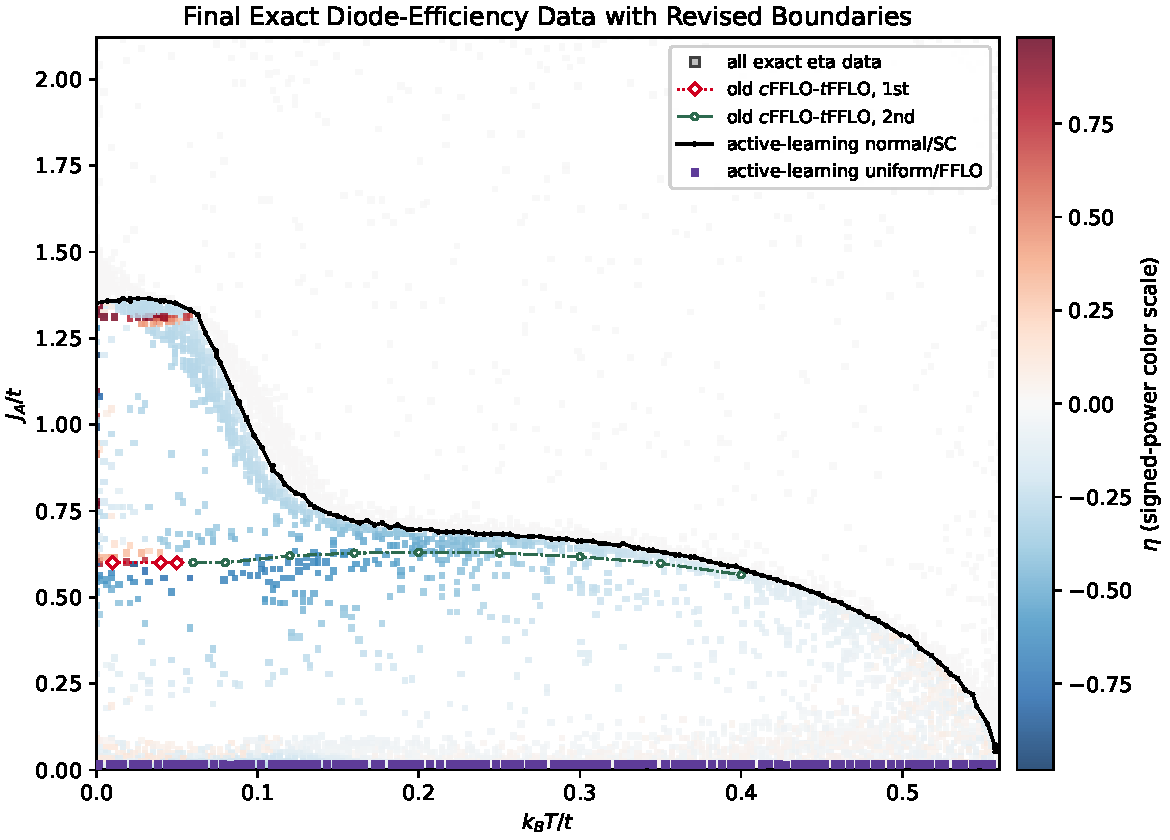
\includegraphics[width=0.88\linewidth]{figures/exact_eta_revised_boundaries.pdf}
  \caption{All exact diode-efficiency data with active-learning revised
  thermodynamic boundaries and the older cFFLO/tFFLO reference curves.  The
  color data should be interpreted with the response-reliability caveats
  discussed below.}
\end{figure}

\begin{figure}[H]
  \centering
  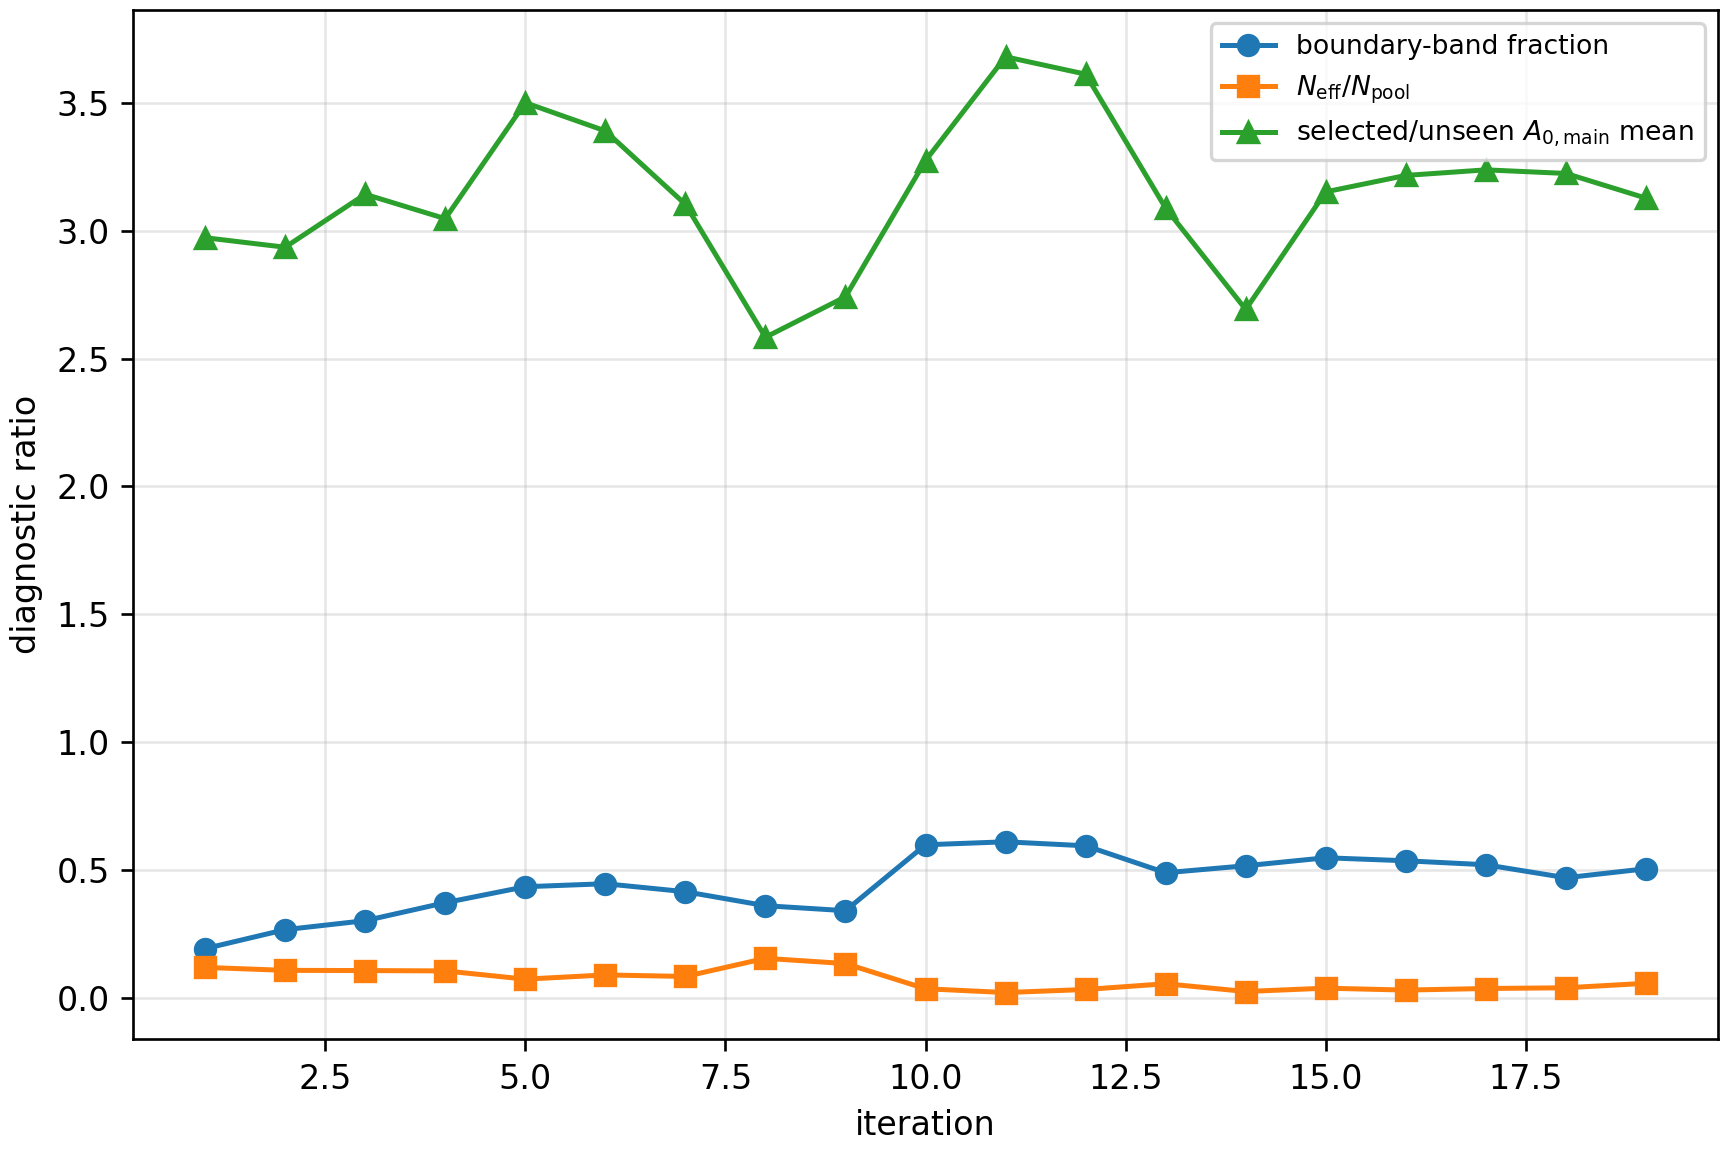
\includegraphics[width=0.78\linewidth]{figures/selection_focus_curve.png}
  \caption{Discovery-mode selection diagnostics.  The active pool and selected
  points became increasingly focused near predicted phase boundaries rather
  than behaving as uniform random coverage.}
\end{figure}

\section*{Delta-refinement and high-\(J_A\) boundary audit}

The first numerical audit isolated high-\(J_A\) normal/SC boundary-kink points,
high-\(J_A\) positive-\(\eta\) points, Delta-ambiguous points, and rerun-required
points.  The Delta refinement subset contained \(92\) rows.  The stricter
Delta refinement changed \(5\) phase labels and left \(4\) boundary-ambiguous
points.  The new strict phase counts were:
\[
N_{\rm normal}=57,\qquad
N_{\rm FFLO}=30,\qquad
N_{\rm boundary\ ambiguous}=4,\qquad
N_{\rm uniform\ SC}=1.
\]

This audit supports the conclusion that some high-\(J_A\) normal/SC boundary
features are tied to near-zero-\(\Delta\) ambiguity rather than a clean, sharply
resolved thermodynamic boundary.  It does not yet close the separate question
of whether a larger \(q\)-window could reveal a lower superconducting branch
outside the original scan.

\section*{Response-level q-window audit for high-\(J_A\) positive \(\eta\)}

The high-\(J_A\), positive-\(\eta\) anomaly audit expanded the \(q\)-window and
recomputed the response.  The complete q-window audit used \(33\) input points
and two expansion levels per point, giving \(66\) q-window rows.  All
\(66/66\) rows passed the response-level q-window validity test:
\[
\text{left endpoint found},\quad \text{right endpoint found},\quad
q_{\rm opt}, q_{I_c^+}, q_{I_c^-}\ \text{away from window edges}.
\]
Thus, for the tested response points, the window width itself is no longer the
dominant uncertainty.

The complete q-window classification was:
\[
57 \ \text{q-window artifacts},\qquad
9 \ \text{response-stable-positive rows}.
\]
At the point level, after the two-level q-window audit:
\[
27 \ \text{points became non-positive},\quad
3 \ \text{changed sign},\quad
2 \ \text{had unstable extrema locations},\quad
1 \ \text{passed the two-level screen}.
\]

\begin{figure}[H]
  \centering
  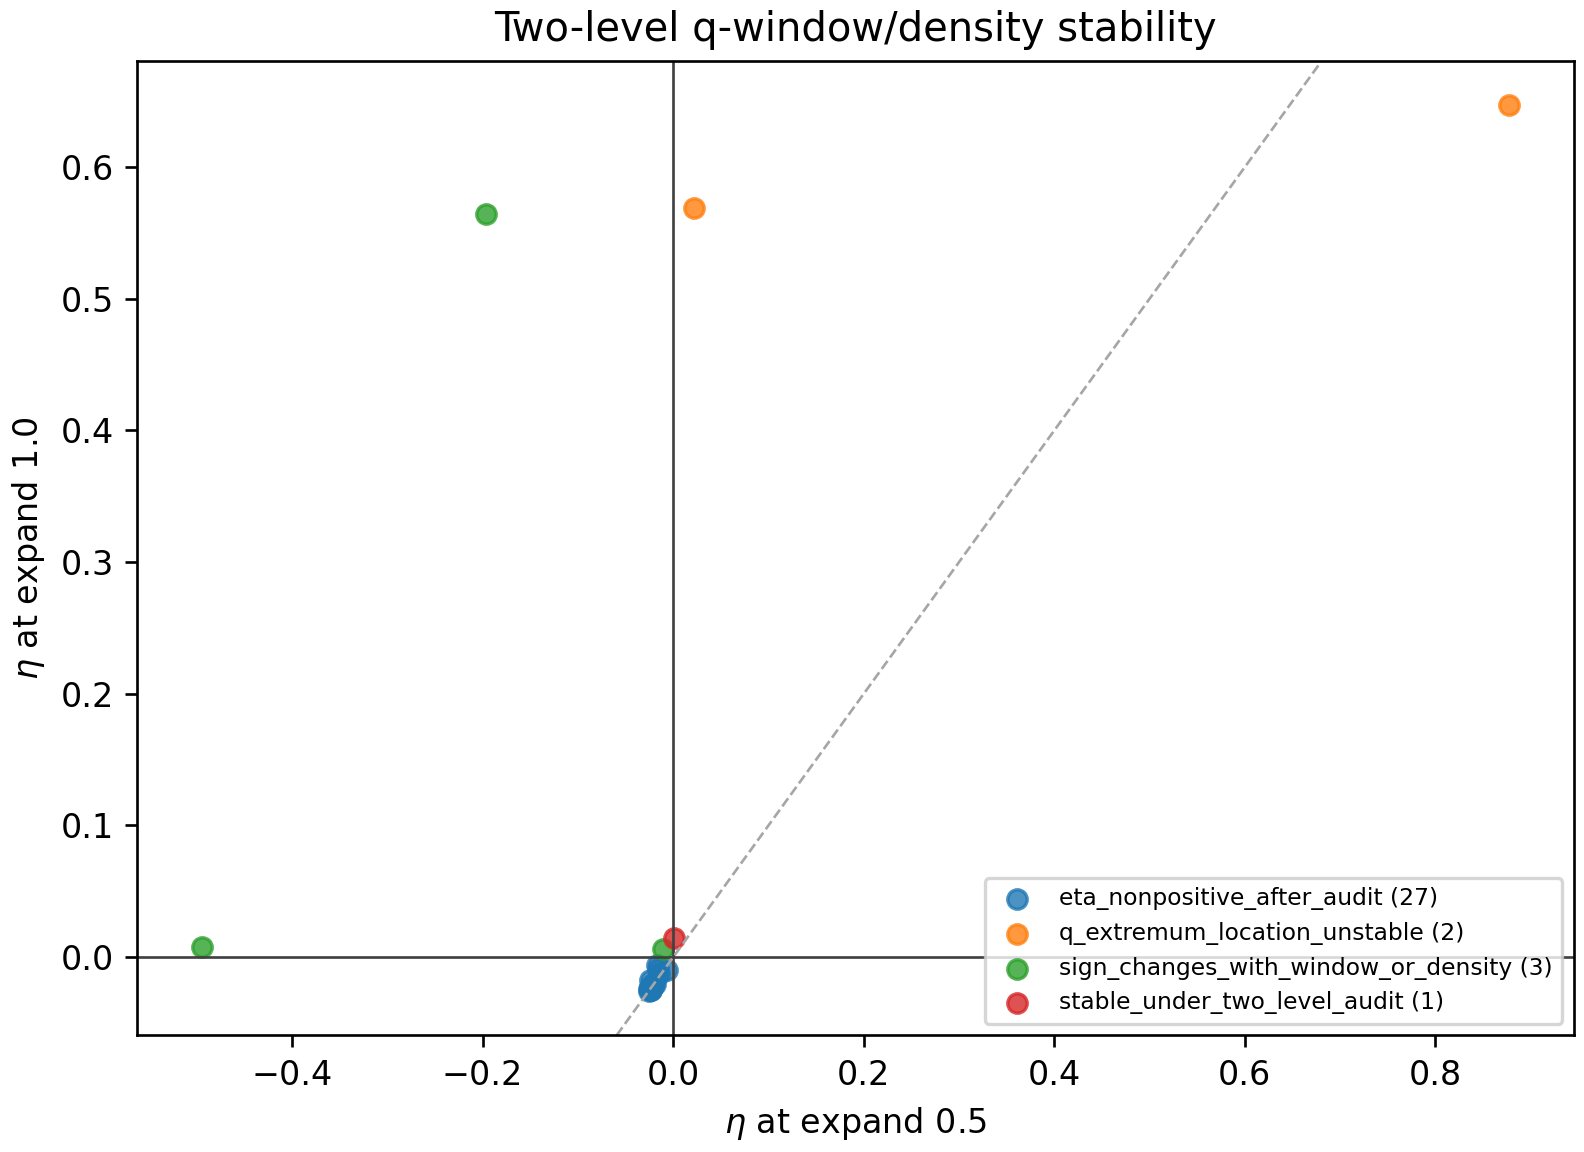
\includegraphics[width=0.78\linewidth]{figures/qwindow_two_level_eta_stability.png}
  \caption{Two-level q-window stability for the originally positive high-\(J_A\)
  response candidates.}
\end{figure}

\begin{figure}[H]
  \centering
  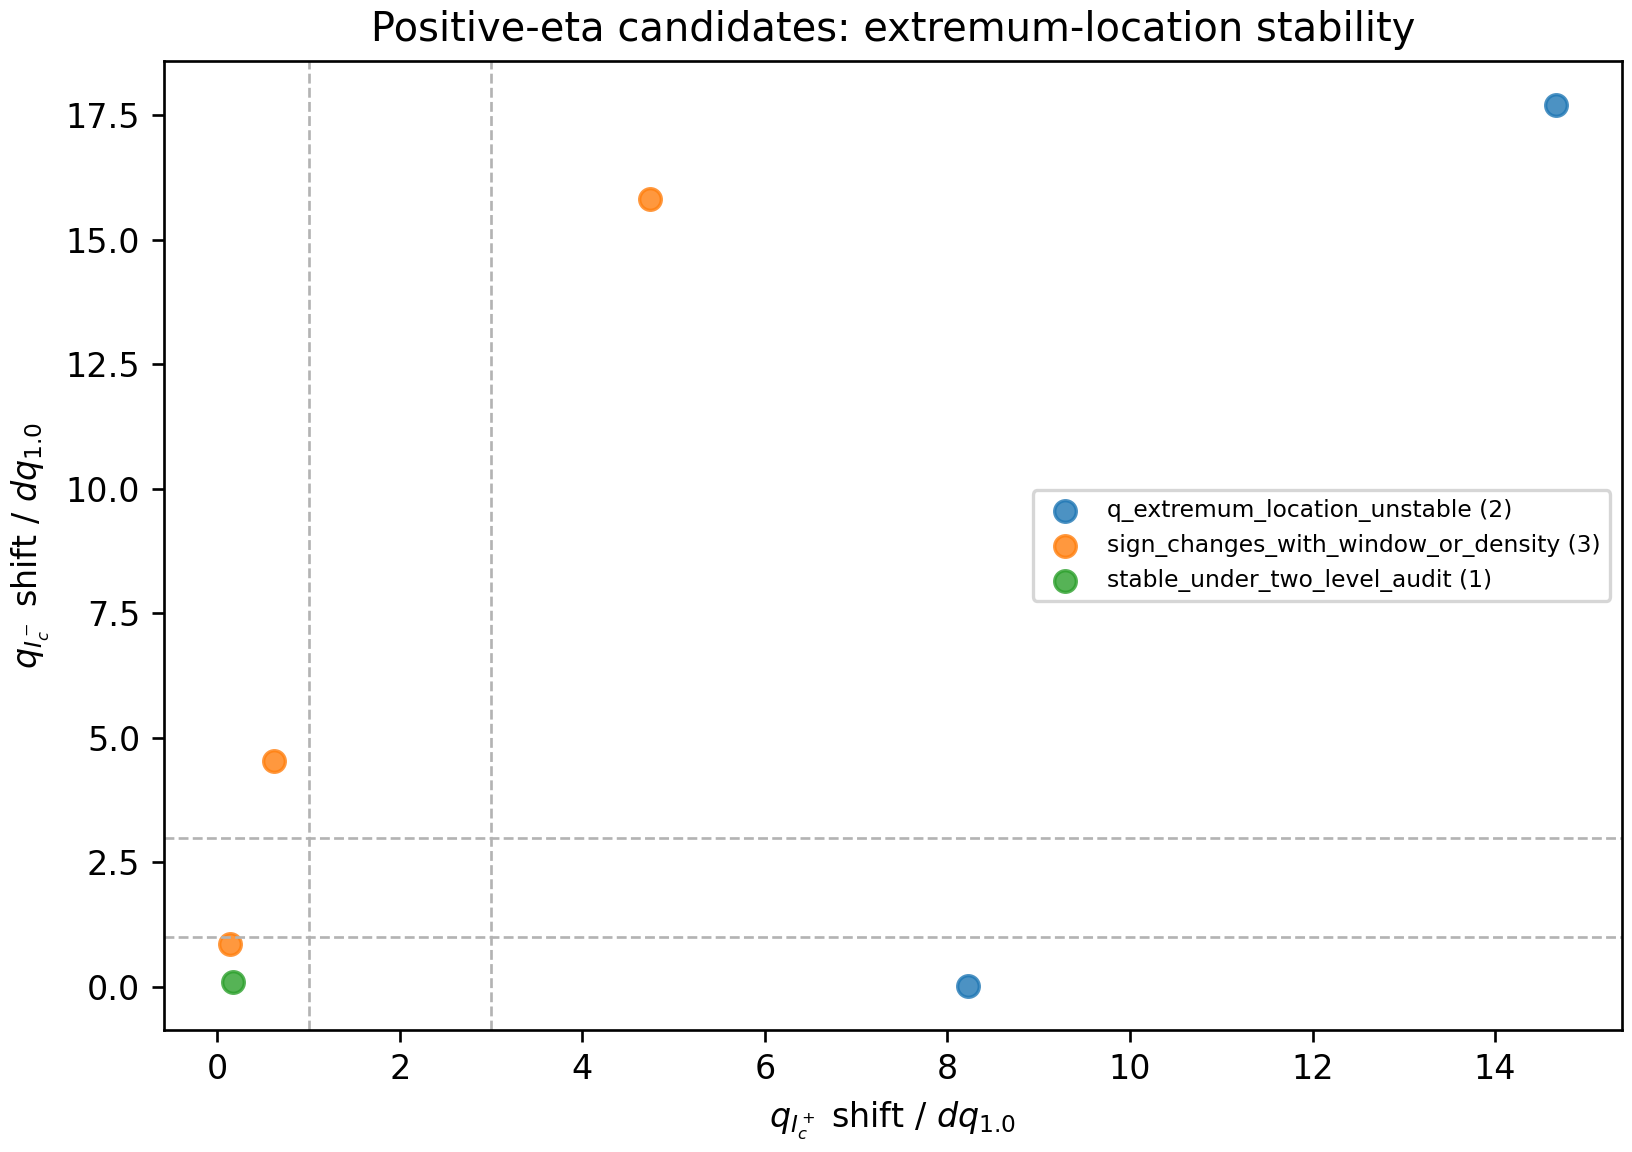
\includegraphics[width=0.78\linewidth]{figures/qwindow_positive_eta_qextrema_shift.png}
  \caption{Critical-current extremum shifts among the remaining positive
  response candidates after q-window expansion.}
\end{figure}

\section*{Fixed-window q-density convergence audit}

After the q-window width was shown to be sufficient, the remaining issue was
q-grid density and response-extremum extraction.  The fixed-window q-density
audit held the \(q\)-window fixed to the expanded \(\texttt{expand\_1.0}\)
range and recomputed six residual candidates:
\[
\text{points } 11, 13, 17, 20, 21, 25,
\qquad n_q=3200,6400,12800.
\]
All \(18/18\) point-density rows returned successfully.

The classification was:
\[
\begin{array}{lr}
\text{density-converged large positive } \eta & 0\\
\text{weak near-zero positive } \eta & 0\\
\text{sign-changing artifact} & 4\\
\text{q-extremum-location unstable} & 1\\
\text{unresolved} & 1
\end{array}
\]

\begin{center}
\begin{tabular}{rrrrlp{0.42\linewidth}}
\toprule
Point & \(k_B T/t\) & \(J_A/t\) & \(\eta_{6400}\) & \(\eta_{12800}\) & Classification\\
\midrule
11 & 0.002333 & 1.33825 & 1 & -1 & sign-changing artifact\\
13 & 0 & 1.344875 & -1 & 1 & sign-changing artifact\\
17 & 0.004667 & 1.32500 & -1 & 1 & sign-changing artifact\\
20 & 0.007000 & 1.35150 & 1 & -1 & sign-changing artifact\\
21 & 0 & 1.33825 & 1 & 1 & unresolved\\
25 & 0 & 1.318375 & 1 & 1 & q-extremum-location unstable\\
\bottomrule
\end{tabular}
\end{center}

\begin{figure}[H]
  \centering
  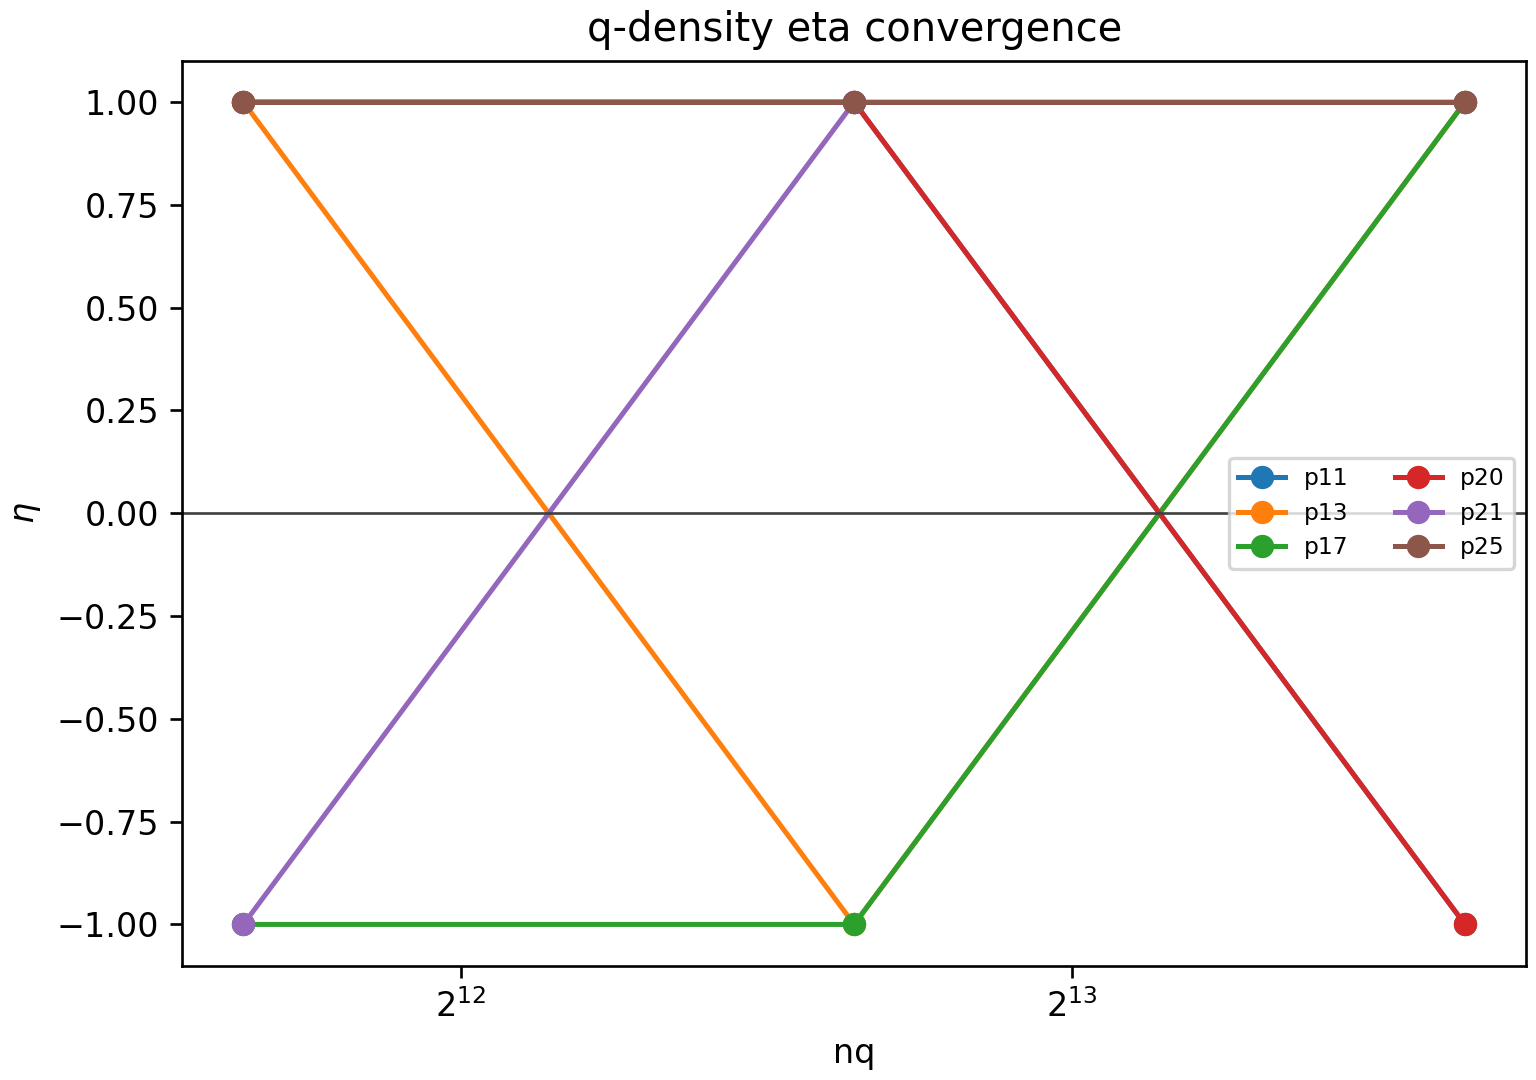
\includegraphics[width=0.78\linewidth]{figures/qdensity_eta_vs_nq.png}
  \caption{Fixed-window \(\eta\) values as the q-grid density is increased.}
\end{figure}

\begin{figure}[H]
  \centering
  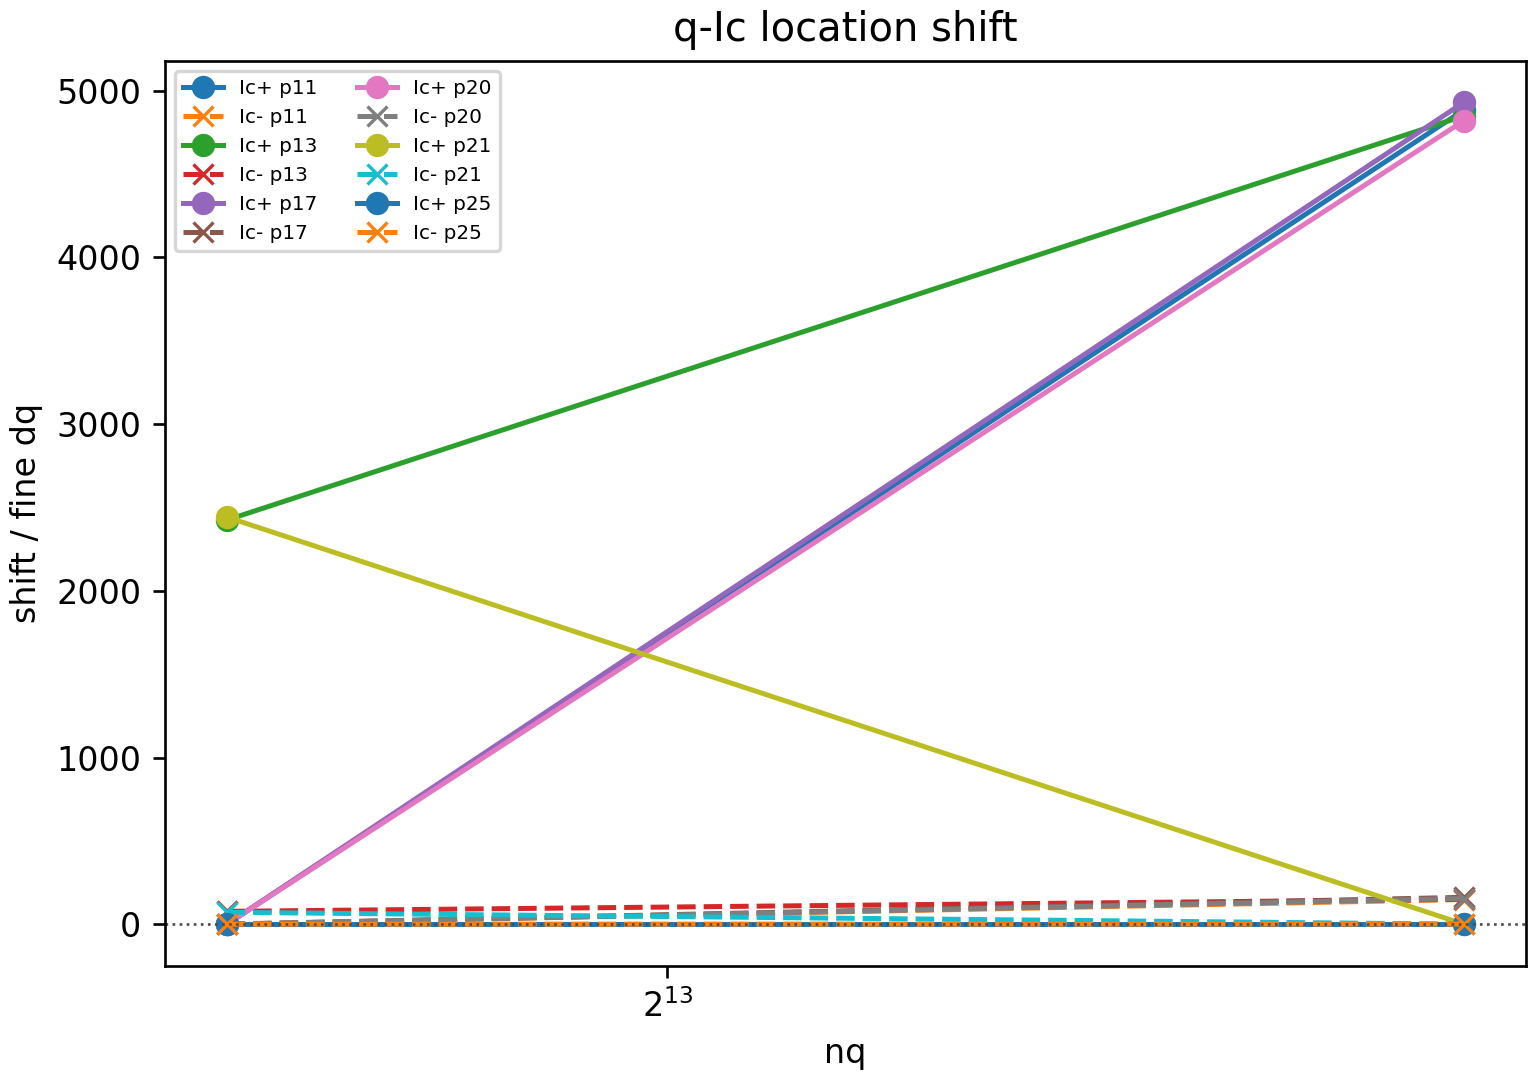
\includegraphics[width=0.78\linewidth]{figures/qdensity_qic_shift_vs_nq.png}
  \caption{Critical-current extremum shifts in units of the finer q-grid
  spacing.}
\end{figure}

This result rules out a robust positive-\(\eta\) conclusion for the six
residual candidates at the current numerical tolerance.  The remaining
\(\eta=1\) cases required direct response-curve inspection.

\section*{Response-curve pathology audit}

The final audit examined full response curves for points \(21\) and \(25\) at
\(n_q=6400,12800\).  For each curve, the saved fields were:
\[
q,\quad \Delta(q),\quad F(q),\quad I(q),\quad \text{branch\_valid\_mask}.
\]
The audit plotted the \(I^+(q)\) and \(I^-(q)\) branches separately and marked
\(q_{I_c^+}\), \(q_{I_c^-}\), \(q_{\rm opt}\), and the superconducting branch
endpoints.  It also recorded the top local extrema of each branch.

\begin{center}
\begin{tabular}{rrrrrl}
\toprule
Point & \(n_q\) & \(I_c^+\) & \(I_c^-\) & \(|I_c^+|+|I_c^-|\) & Pathology\\
\midrule
21 & 6400 & \(7.38\times10^{-5}\) & 0 & \(7.38\times10^{-5}\) & small denominator\\
21 & 12800 & \(2.57\times10^{-4}\) & 0 & \(2.57\times10^{-4}\) & branch near zero\\
25 & 6400 & \(2.07\times10^{-4}\) & 0 & \(2.07\times10^{-4}\) & branch near zero\\
25 & 12800 & \(3.77\times10^{-5}\) & 0 & \(3.77\times10^{-5}\) & small denominator\\
\bottomrule
\end{tabular}
\end{center}

The response rule used here is conservative: if
\[
|I_c^+|+|I_c^-| < 10^{-4},
\]
or if either branch is numerically zero, \(\eta\) is marked ill-conditioned and
is not allowed as a positive diode-response claim.

\begin{figure}[H]
  \centering
  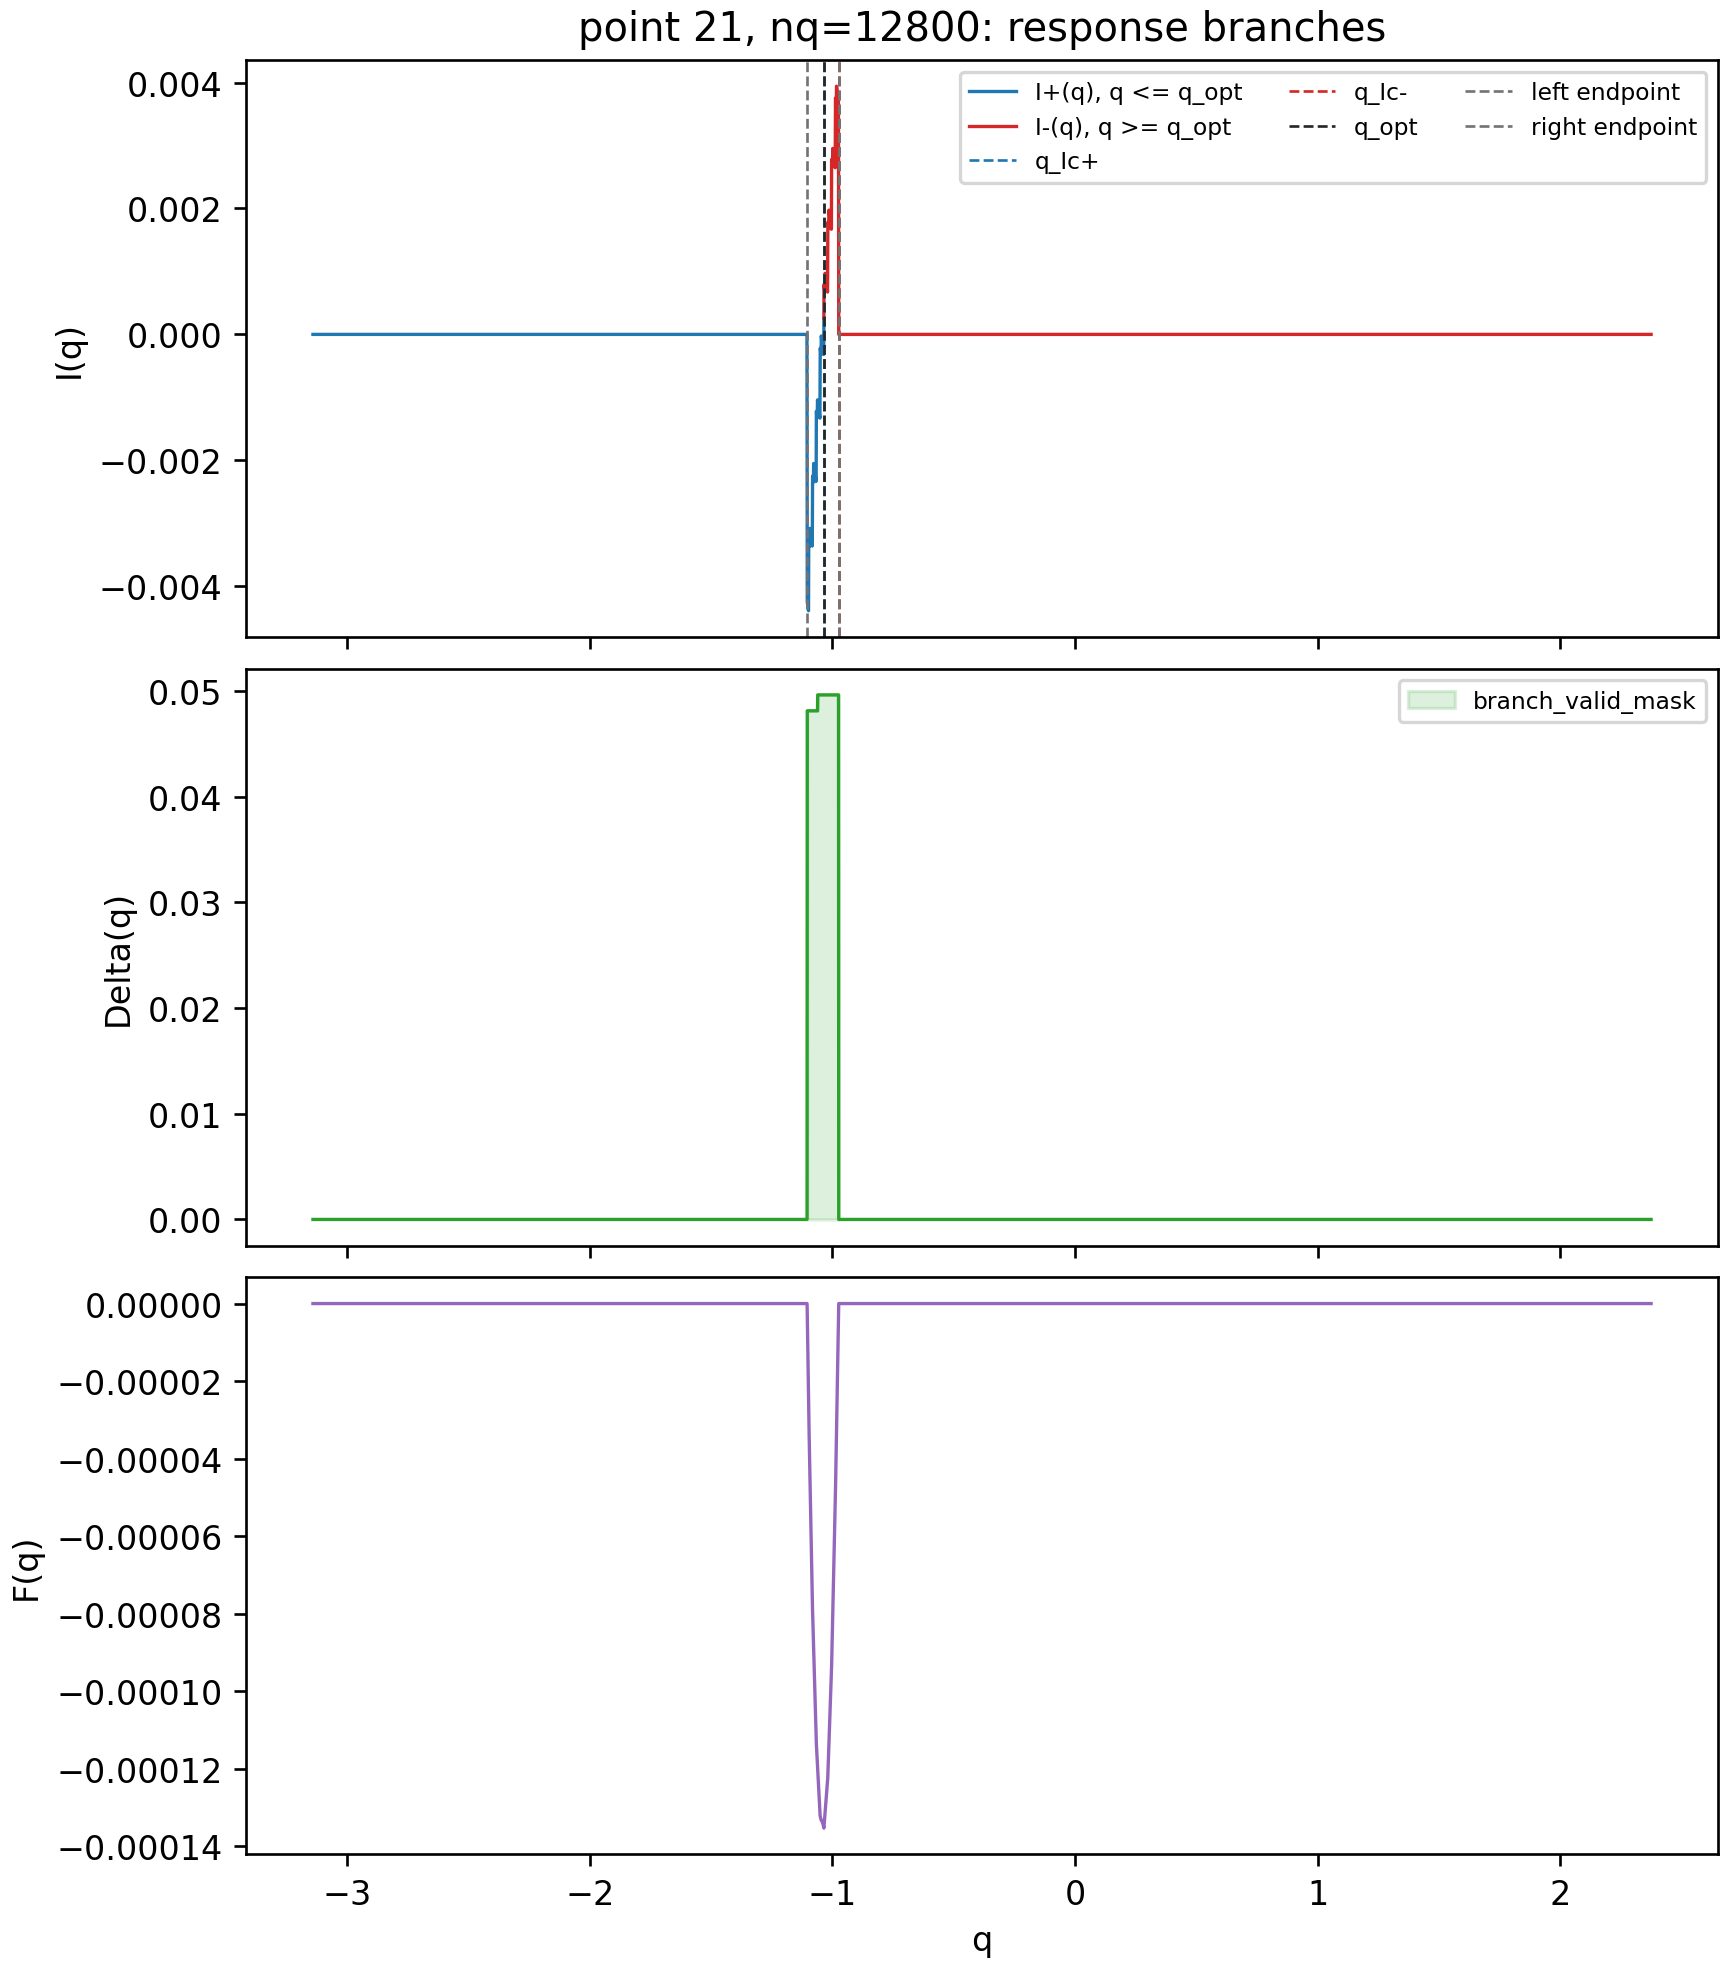
\includegraphics[width=0.86\linewidth]{figures/point0021_nq12800_response_pathology.png}
  \caption{Response-curve pathology audit for point 21 at \(n_q=12800\).}
\end{figure}

\begin{figure}[H]
  \centering
  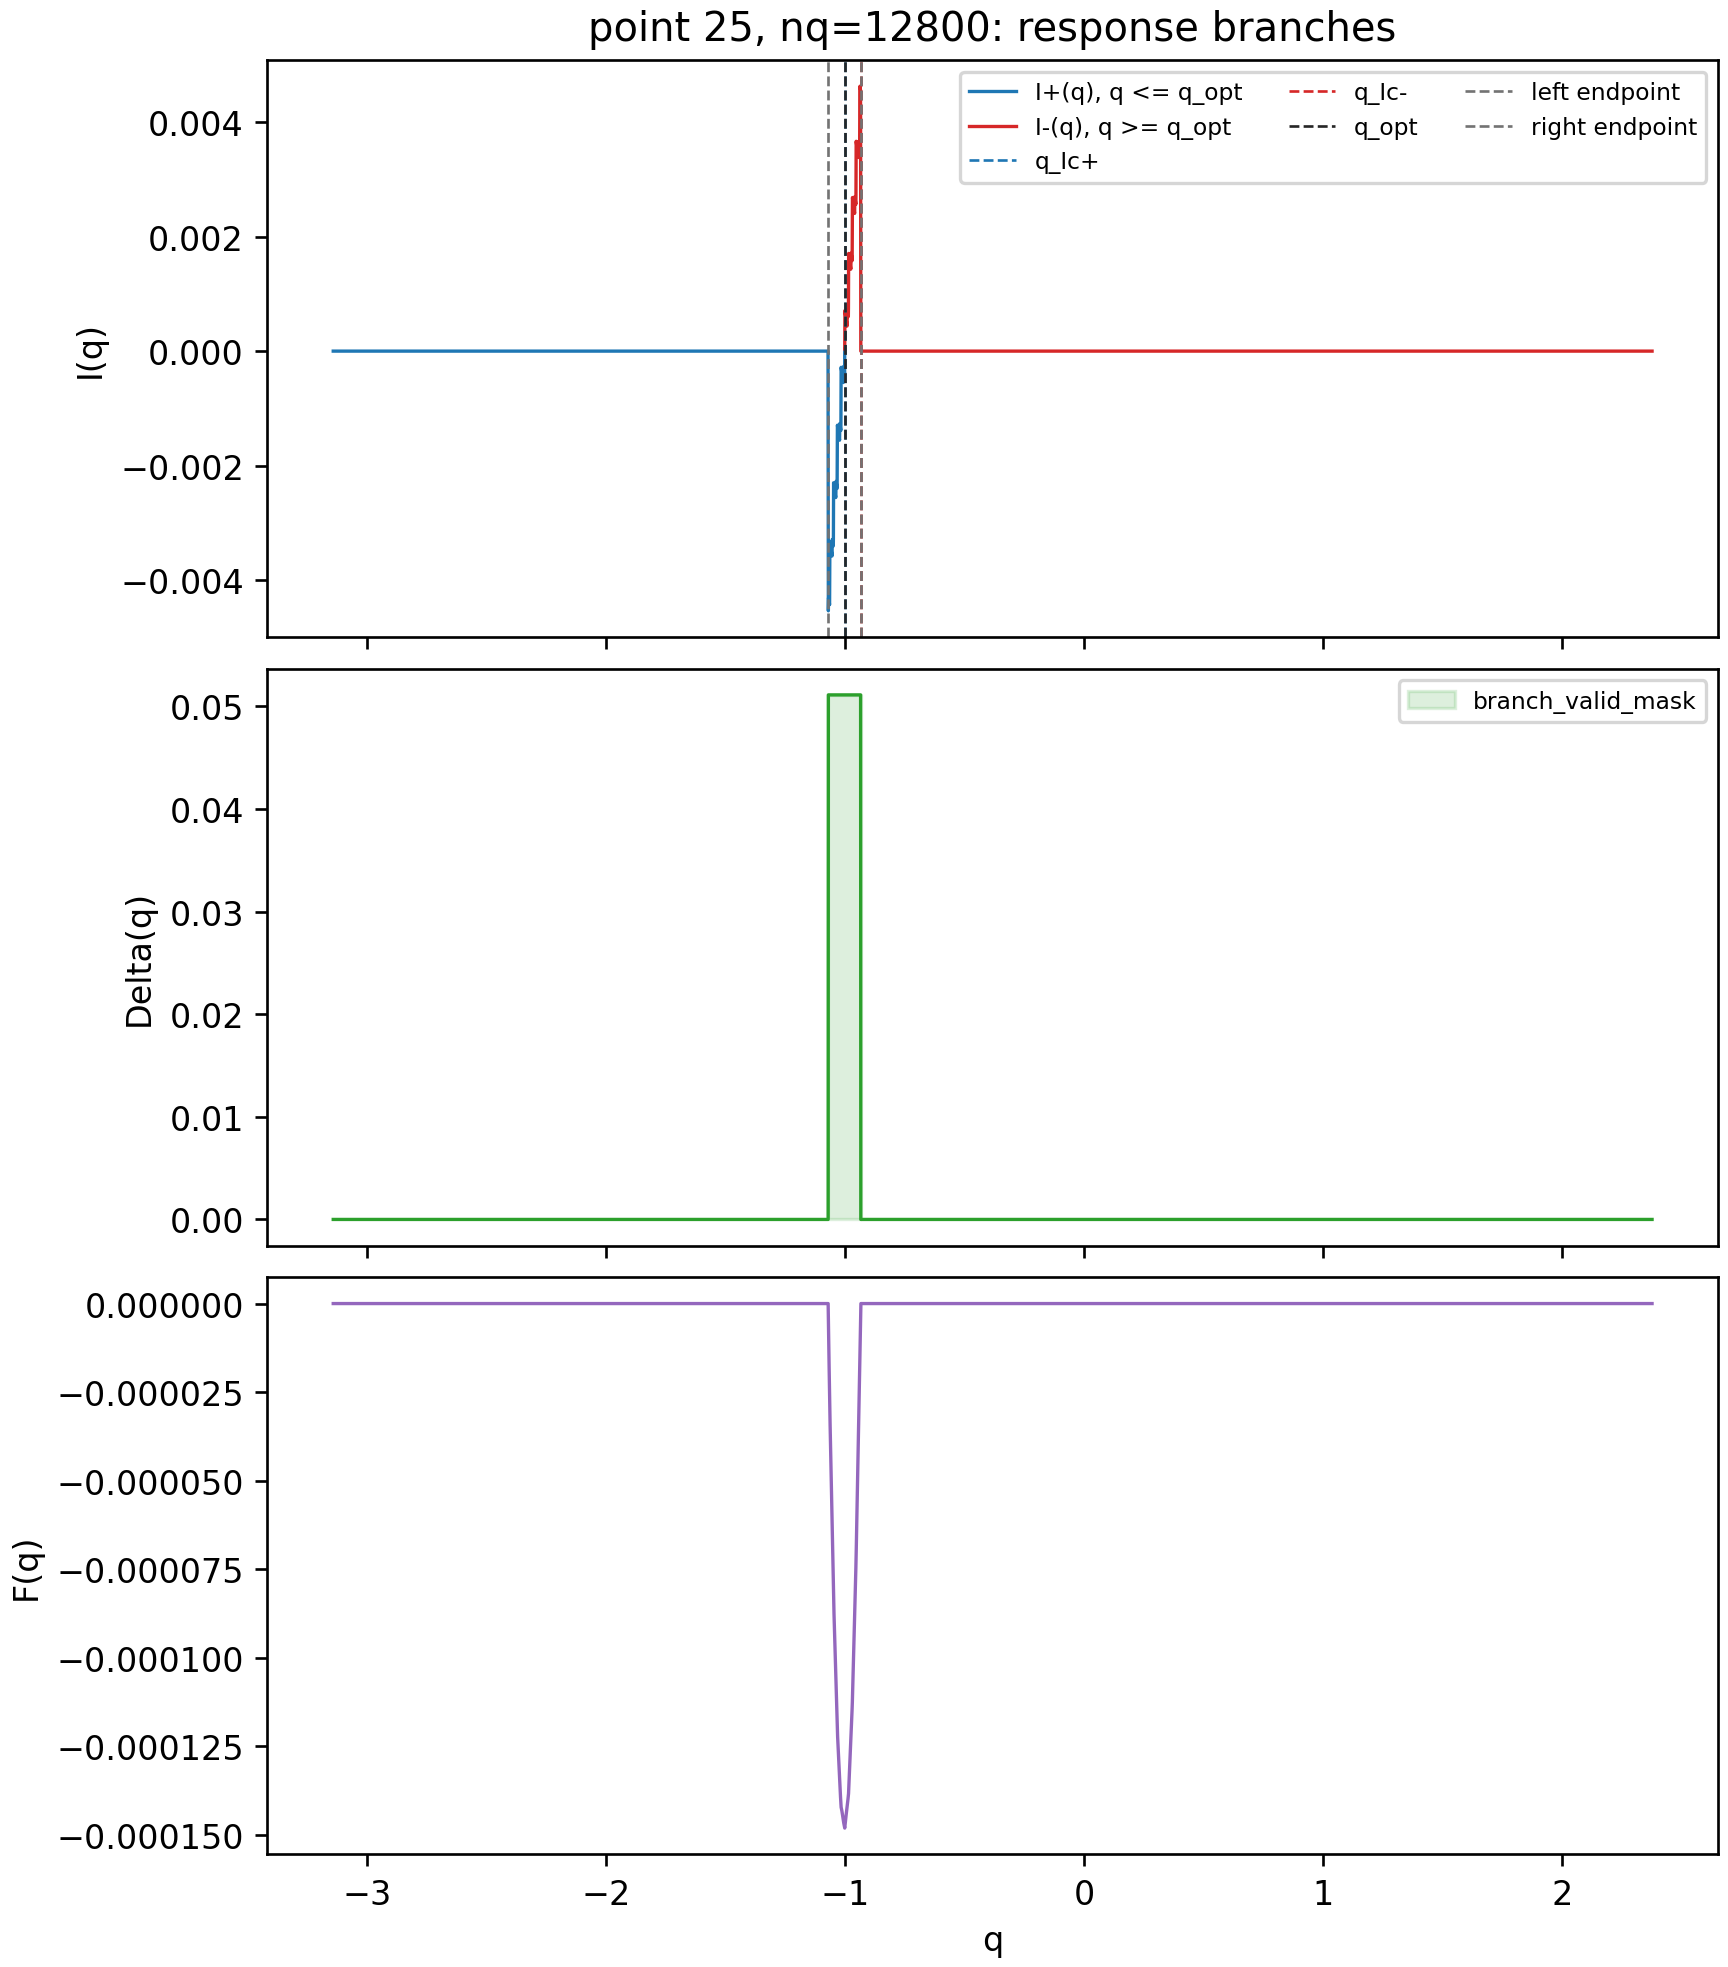
\includegraphics[width=0.86\linewidth]{figures/point0025_nq12800_response_pathology.png}
  \caption{Response-curve pathology audit for point 25 at \(n_q=12800\).}
\end{figure}

Both point 21 and point 25 have \(\eta=1\) only because \(I_c^-=0\).  They must
therefore be reported as
\[
\eta\ \text{ill-conditioned / branch-near-zero},
\]
not as robust positive-\(\eta\) physics.

\section*{Current interpretation}

The numerical audits support the following working interpretation:

\begin{enumerate}
  \item The discovery active-learning workflow found the main thermodynamic
        normal/SC and uniform-SC/FFLO boundary structure.
  \item The free-energy phase criterion is internally consistent within the
        scanned \((\Delta,q)\) window.
  \item The high-\(J_A\), positive-\(\eta\) points are not stable diode-response
        evidence.  Most disappear or change sign after q-window and q-density
        audits; the remaining \(\eta=1\) points are small-denominator or
        branch-near-zero pathologies.
  \item The dominant remaining uncertainty for the thermodynamic phase diagram
        is not the \(\eta\) response.  It is whether the high-\(J_A\), low-\(T\)
        free-energy scan covers all relevant FFLO branches.
  \item The normal/SC boundary near high \(J_A\) also needs sharper
        near-zero-\(\Delta\) refinement, because several boundary points remain
        close to the normal-state energy within numerical tolerance.
\end{enumerate}

\section*{Open problems and next calculation}

The most important unresolved calculation is a phase-boundary q-window and
branch-minimum audit.  This is distinct from the response-level \(\eta\) audit.
For selected high-\(J_A\), low-\(T\), normal/SC-kink points, the next audit
should:

\begin{enumerate}
  \item expand the q-window for the free-energy scan,
  \item save \(F_{\min}(q)=\min_\Delta F(\Delta,q)\),
  \item extract multiple low-energy local minima, not only the global minimum,
  \item compare old and expanded-window phase labels, \(q_{\rm opt}\),
        \(\Delta_{\rm opt}\), and \(\Delta F\),
  \item identify whether a lower FFLO branch appears outside the old window,
  \item only then decide whether the high-\(J_A\) normal/SC boundary is stable.
\end{enumerate}

Topology remains another open layer.  The old cFFLO/tFFLO reference curves are
not pointwise topological labels from the current exact oracle.  A final
topological phase diagram requires evaluating the topological invariant for
each relevant low-energy FFLO local minimum, not just for the final global
\(q_{\rm opt}\) state.

\section*{Report artifacts}

This note summarizes data from:

\begin{itemize}
  \item \texttt{numerical\_audit\_qwindow\_delta\_v1\_result2}
  \item \texttt{numerical\_audit\_qdensity\_v1}
  \item \texttt{numerical\_audit\_qdensity\_v1/response\_curve\_pathology\_audit}
\end{itemize}

The copied CSV tables in \texttt{tables/} contain the fixed-window q-density
summary and the final response-pathology summary.

\end{document}
